% Fichier généré automatiquement par tools/generate_corrections.py.
% Source : GEO/GEO-01/12_BielleManivelle/12_BielleManivelle.tex
% Statut : complété (4/4 question(s)).
\begin{corrigebox}[Corrigé complété]
\CorrigeQuestion{1}
\CorrigeSource{Réponse reprise d'un exercice homonyme de la banque ; la provenance exacte est indiquée dans le commentaire du fichier.}
% Réponse reprise de : GEO/GEO-03/12_BielleManivelle/12_BielleManivelle.tex
\begin{marginfigure}
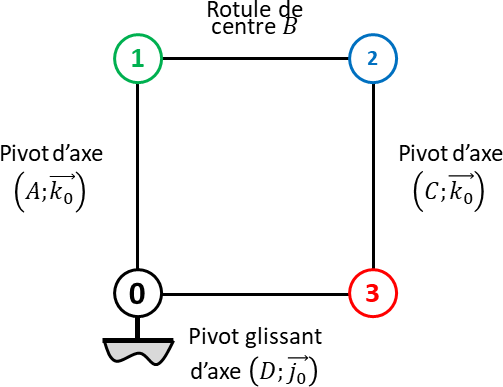
\includegraphics[width=\linewidth]{../../GEO-03/12_BielleManivelle/images/12_01_c}
\end{marginfigure}
\CorrigeQuestion{2}
On reconstruit la configuration en appliquant les
                rotations dans l'ordre de la chaîne cinématique puis les translations le
                long de leurs axes. Les longueurs des barres restent constantes. Les
                coordonnées finales se calculent avec
                $\vec i'=\cos q\,\vec i+\sin q\,\vec j$; le tracé doit conserver les
                liaisons et le contact sans pénétration.
\CorrigeQuestion{3}
On reconstruit la configuration en appliquant les
                rotations dans l'ordre de la chaîne cinématique puis les translations le
                long de leurs axes. Les longueurs des barres restent constantes. Les
                coordonnées finales se calculent avec
                $\vec i'=\cos q\,\vec i+\sin q\,\vec j$; le tracé doit conserver les
                liaisons et le contact sans pénétration.
\CorrigeQuestion{4}
On reconstruit la configuration en appliquant les
                rotations dans l'ordre de la chaîne cinématique puis les translations le
                long de leurs axes. Les longueurs des barres restent constantes. Les
                coordonnées finales se calculent avec
                $\vec i'=\cos q\,\vec i+\sin q\,\vec j$; le tracé doit conserver les
                liaisons et le contact sans pénétration.
\end{corrigebox}
